\subsubsection{Odabir plana ishrane}

\begin{figure}[H]
\begin{center}
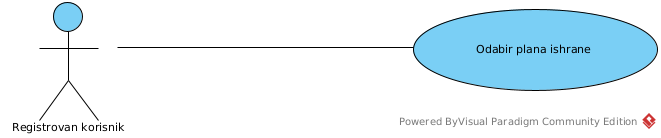
\includegraphics[width=\textwidth]{Pictures/uc_select_meal_plan.png}
\end{center}
    \caption{Dijagram slučaja upotrebe odabira plana ishrane}
\label{fig:UCSelectMealPlan}
\end{figure}

\begin{itemize}
    \item Kratak opis:
        \begin{itemize}
            \item Registrovani korisnik bira svoj plan ishrane 
        \end{itemize}
    \item Učesnici:
        \begin{itemize}
            \item Registrovan korisnik
        \end{itemize}
    \item Preduslovi:
        \begin{itemize}
            \item Sistem je u ispravnom stanju
            \item Korisnik mora biti registrovan i ulogovan na aplikaciju
            \item Korisnik se prvi put ulogovao na aplikaciju
        \end{itemize}
    \item Postuslovi:
        \begin{itemize}
            \item Podaci su uspešno sačuvani u bazi podataka, zakazana je dostava hrane i skinut je novac sa računa za prvu nedelju
        \end{itemize}
    \item Osnovni tok:
        \begin{enumerate}
            \item Sistem prikazuje korisniku formu za odabir plana
            \item Korisnik bira svoje preference za tip obroka za koji želi da dobija recepte
            \item Korisnik bira za koliko osoba će biti obrok
            \item Korisnik bira koliko obroka u nedelji želi
            \item Sistem prikazuje korisniku cenu odabranog plana
            \item Korisnik potvrđuje odabir plana
            \item Sistem prikazuje korisniku formu za unos adrese, željenog dana dostave i satnice dostave
            \item Korisnik potvđuje podatke koje je uneo
            \item Sistem prikazuje korisniku recepte koje može odabrati
            \item Korisnik bira recepte
            \item Sistem prikazuje korisniku formu za unos detalja o plaćanju
            \item Korisnik potvrđuje svoje podatke o plaćanju i potvrđuje narudžbinu
            \item Sistem čuva podatke i skida novac sa korisnikovog računa
            \item Sistem prikazuje poruku o uspešnosti 
        \end{enumerate}
    \item Alternativni tok:
        \begin{itemize}
            \item Pad sistema. Ukoliko sistem prestane sa radom u bilo kom trenutku, prelazi se na slučaj upotrebe ``Pravljenje rezervne kopije i oporavak baze podataka''.
            \item Ukoliko sistem u 13. koraku ne uspe da obavi skidanje novca sa računa, obaveštava korisnika o tome sa porukom o grešci. Proces se nastavlja u 11. koraku osnovnog toka.
        \end{itemize}
    \item Dodatne informacije:
        \begin{itemize}
            \item Preference za tip obroka su: obroci zasnovani na mesu i povrću, obroci zasnovani na povrću, obroci namenjeni korišćenju od strane porodice, obroci kod kojih se pazi na broj kalorija, brzi i jednostavni obroci i obroci zasnovani na pesketarijanskoj ishrani 
            \item Obrok može biti za 2 ili 4 osobe
            \item Moguće je odbrati od 2 do 6 obroka u nedelji
        \end{itemize}
\end{itemize}

\begin{figure}[H]
\begin{center}
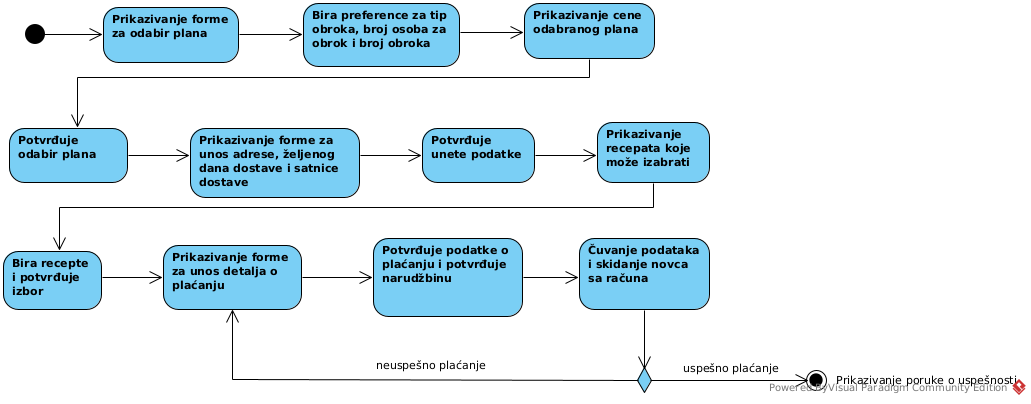
\includegraphics[width=\textwidth]{activity_select_meal_plan.png}
\end{center}
    \caption{Dijagram aktivnosti odabira plana ishrane}
\label{fig:ActivitySelectMealPlan}
\end{figure}
